\documentclass[10pt,pdf,hyperref={unicode}]{beamer}

\usepackage[utf8]{inputenc}
\usepackage[russian]{babel}
\usepackage{amssymb,amsmath}
\textwidth=10.7cm % ширина текста


\usepackage{color}
\usepackage{url}

\usepackage{indentfirst}
\usepackage{graphicx}

\usetheme{Warsaw}%Goettingen}


\title{\small{Выпускная квалификационная работа}}
\subtitle{\large{Построение ансамбля алгоритмов рекомендаций}}

%\author{Кудрявцев Георгий}
\institute{\begin{flushright}
      \parbox{0.5\textwidth}{
        \raggedleft
        \textbf{Выполнил:}\\
        студент 417 группы\\
        Кудрявцев Георгий Алексеевич\\[5mm]
        \textbf{Научный руководитель:}\\
        д.ф-м.н., профессор\\
        Дьяконов Александр Геннадьевич
      }
    \end{flushright}}
\date{\today}
\begin{document}
\frame{\titlepage}
%\AtBeginSection{
%    \begin{frame}
%        \frametitle{Содержание}
%        \tableofcontents[currentsection]
%        \end{frame}
%}

\begin{frame}{Неформальная постановка задачи}
Требуется улучшить качество работы алгоритмов ранжирования при помощи ансамблирования уже существующих методов.
\end{frame}

\begin{frame}{Предметная область}
 Рассматривается задачи ранжирования по данным с двоичной релевантностью.
 
 На практике данная задача решается при помощи алгоритмов машинного обучения.
 
 В данной работе рассматриваются факторизационные методы и их линейные ансамбли.
\end{frame} 

\begin{frame}{Актуальность задачи}

Построение рекоммендаций для:

\begin{itemize}
\item социальных сетей

\item сайтов знакомств

\item интернет магазинов
\end{itemize}
\end{frame}

\begin{frame}{Цель и задачи}
Цель: разработать метод ансамблирования, который стабильно улучшает качество ранжирования.

Задачи: 

\begin{itemize}
\item Составить обзор современных факторизационных методов ранжирования. 

\item Предложить эффективный метод ансамблирования.

\item Реализовать методы и провести их сравнительный анализ.

\end{itemize}
\end{frame}

\begin{frame}{Формальная постановка задачи}

\textbf{Входные данные}:

 матрица $R$ размера $M \times N$, где $M$ - количество пользователей, $N$ - количество предметов. $R_{ui}$ = 1, если пользователей $u$ взаимодействовал с предметов $i$. В противном случае $R_{ui}$ = 0.

\textbf{Выходные данные}: 

Для каждого пользователя $u$ ранжированный список предметов, которые не лежат в тренировочной выборке.
\end{frame}

\begin{frame}{Обзор существующих методов}

\begin{itemize}
\item \textbf{CLiMF}\footnote{Yue Shi, Alexandros Karatzoglou, Linas Baltrunas.
CLiMF: learning to maximize reciprocal rank with collaborative less-is-more filtering. 2012}
 -- Факторизационный метод, который оптимизирует сглаженную версию метрики MRR.
  	
\item \textbf{MPR\_MF}\footnote{Steffen Rendle, Christoph Freudenthaler, Zeno Gantner.    
         BPR: Bayesian Personalized Ranking from Implicit Feedback. 2009}
-- Факторизационный метод, который оптимизирует AUC.
\item \textbf{TFMAP}\footnote{Yue Shia,Alexandros Karatzogloub, Linas Baltrunas.
TFMAP: Optimizing MAP for Top-N Context-aware Recommendation. 2012} 
-- Факторизационный метод, который оптимизирует сглаженную метрику MAP.
\item \textbf{iMF}\footnote{Yifan Hu, Yehuda Koren, Chris Volinsky.
	Collaborative Filtering for Implicit Feedback Datasets. 2008}
-- Факторизационный метод, который оптимизирует взвешенную квадратичную ошибку.
\end{itemize}
\end{frame}

\begin{frame}{Линейный ансамбль}
Пусть имеется множество базовых алгоритмов $b_i(x)$. 

Необходимо подобрать такие веса $\alpha_i$, чтобы линейная комбинация алгоритмов $\hat{b}(x) = \sum_i \alpha_i b_i(x)$ показывала лучший результат по какому-нибудь заданному функционалу. 
\end{frame}

\begin{frame}{Оптимальное взвешенное голосование}

 Рассмотрим линейную комбинацию двух алгоритмов ранжирования  в следующем виде:
\begin{equation*}
	\hat{f}_{ui} = \alpha f_{ui}^{m_1} + (1 - \alpha) f_{ui} ^ {m_2} \textrm{\ , где $0 \leq \alpha \leq 1$}
\end{equation*} 
	
\begin{figure}[h]
\center{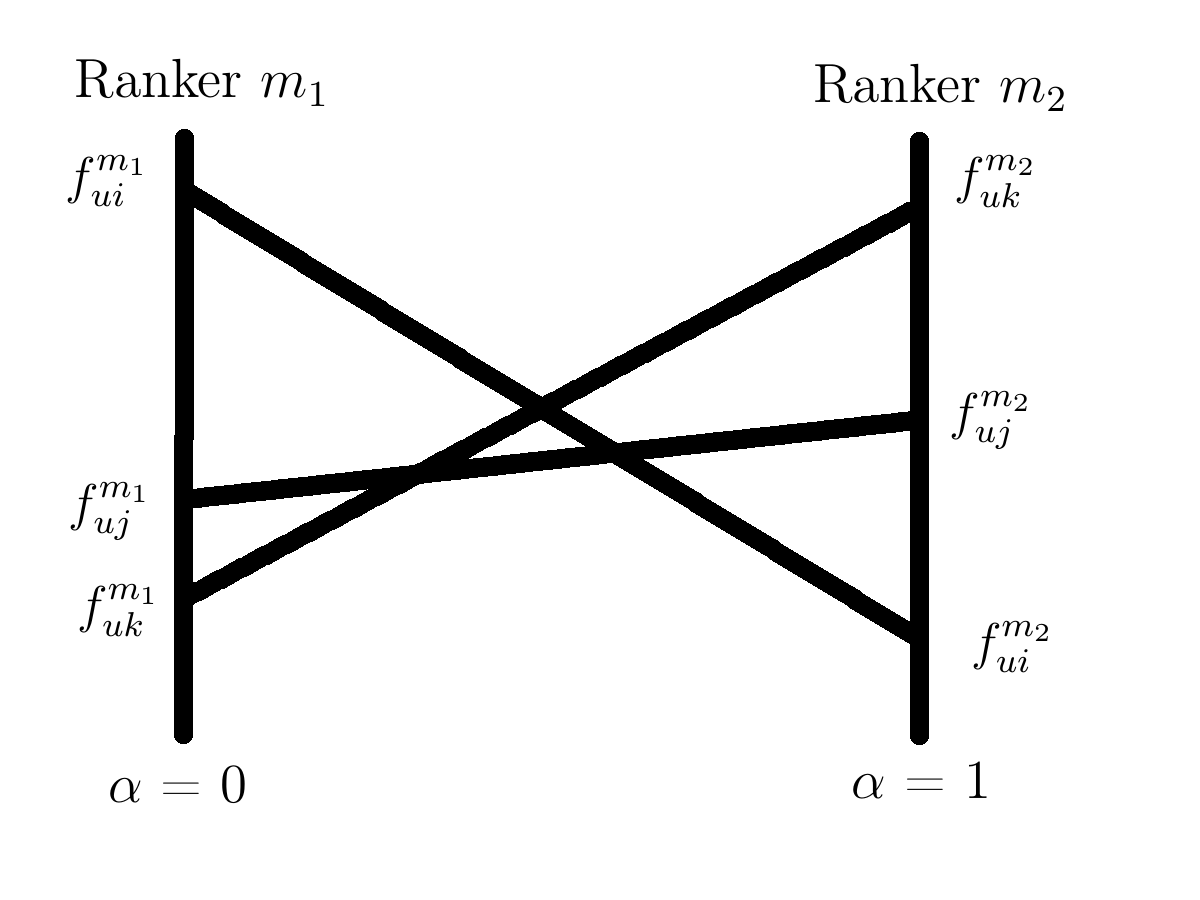
\includegraphics[width=0.4\linewidth]{latexpic}}
\caption{Две вертикальные линии обозначают размер величины f. Чем выше точка, тем больше величина. Невертикальные линии обозначают линейные комбинации величин f. Если $\alpha$ = 0, то линейная комбинация учитывает только Ranker $m_1$, если $\alpha = 1$, то  линейная комбинация учитывает только Ranker $m_2$}
\label{pic:latexpic}
\end{figure}

\end{frame}


\end{document}





